\section{Evaluation}
\subsection{Testing}\label{sec:testing}
Testing has been accomplished by providing a random\_numbers.py file. With three
separate integer parameters, it creates a random list using Python's standard
random library. The inputs include a lower and upper bound as well as a length.
Once the list is created, running make will create a .elf file, which contains
the parallel merge sort algorithm with the unsorted list hard-coded within. Once
the .elf file is loaded on a RISC-V processor, it will immediately begin sorting
the hard-coded list. The implementation also needs the value NUM\_CORES defined
within the Makefile, where it both defines a constant NUM\_CORES for the .elf
file to use, and the same value is used for running the QEMU virtual machine.

This gives the following work flow for creating and running a test:
\begin{itemize}
\item Change directory to src/bare\_metal.
\item Run random\_numbers.py to generate alist.c with an unsorted list.
\item Change the NUM\_CORES variable in the Makefile to the desired number of
  cores.
\item Run "make clean" to remove all files built with previous settings.
\item Run "make test" to generate the .elf file and host QEMU. This step will
  create a test.txt file, as the stdout of QEMU is redirected to said file.
\item Run "python3 validate.py". This reads the test.txt file, first reading the
  unsorted array and sorting that with pythons standard sorting algorithm. Then
  it reads the sorted array from the test.txt file and compares it with pythons
  sorted array.
\end{itemize}

\subsubsection*{Debugging}
\begin{figure}
  \centering
  \begin{subfigure}[b]{0.45\textwidth}
    \centering
    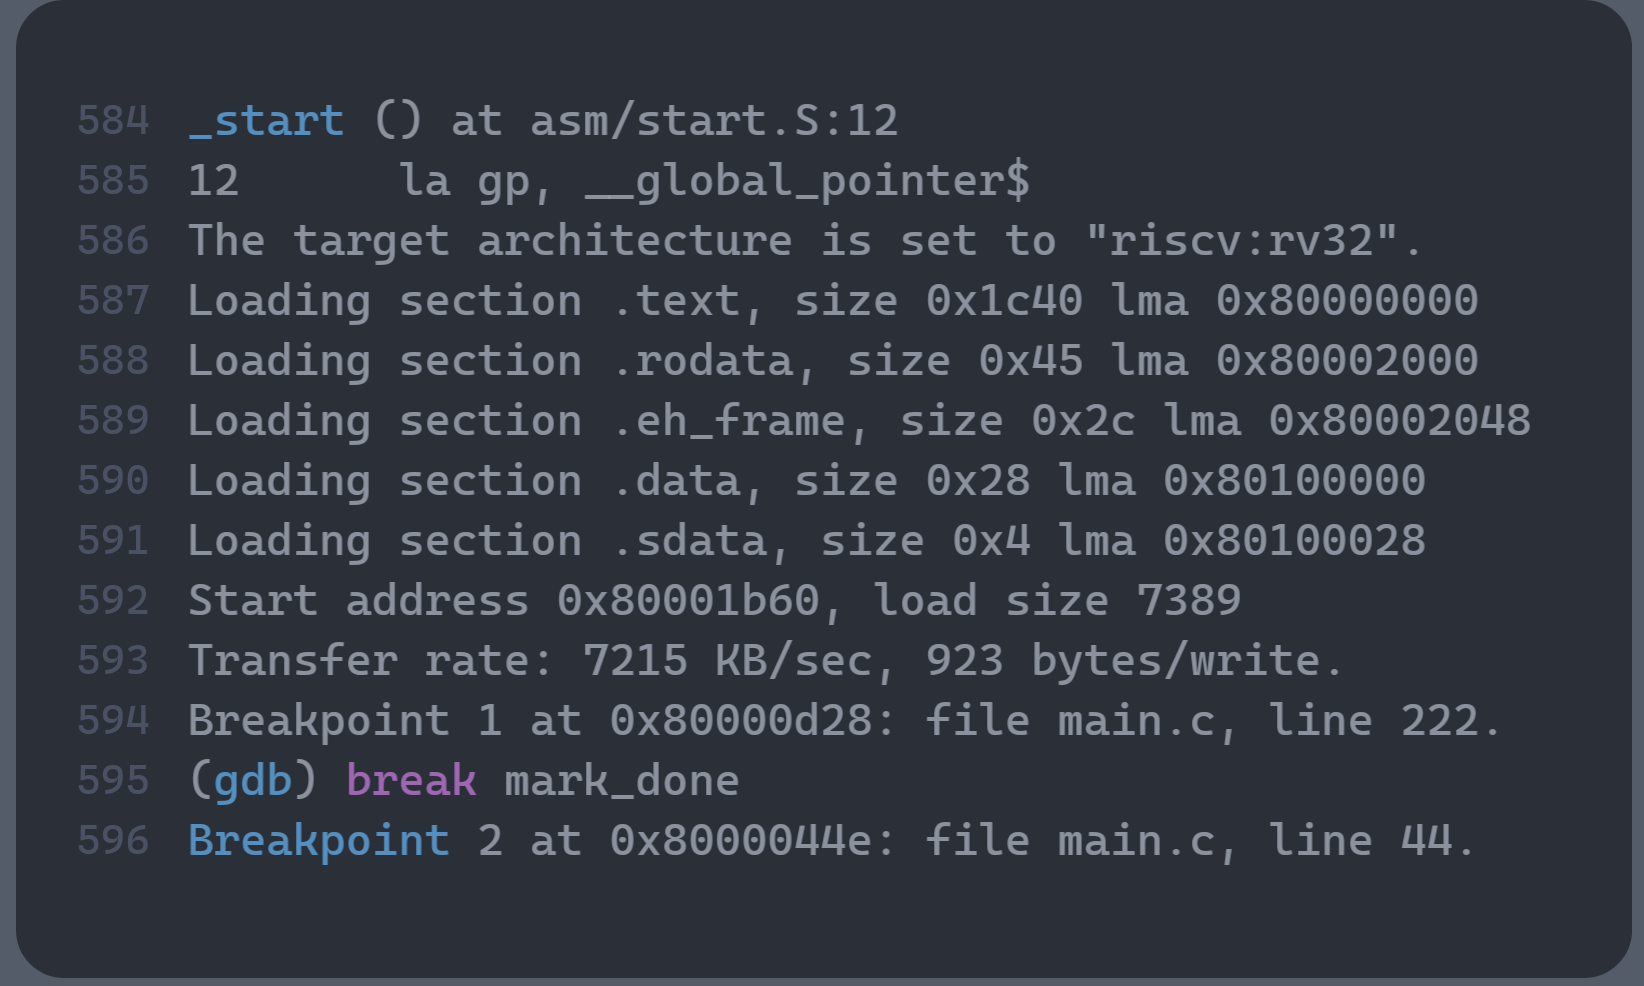
\includegraphics[width=\textwidth]{./figures/debug1.png}
    \caption{Connecting gdb by running "riscv32-unknown-elf-gdb" and breaking at
    mark\_done"}
  \end{subfigure}
  \hfill
  \begin{subfigure}[b]{0.45\textwidth}
    \centering
    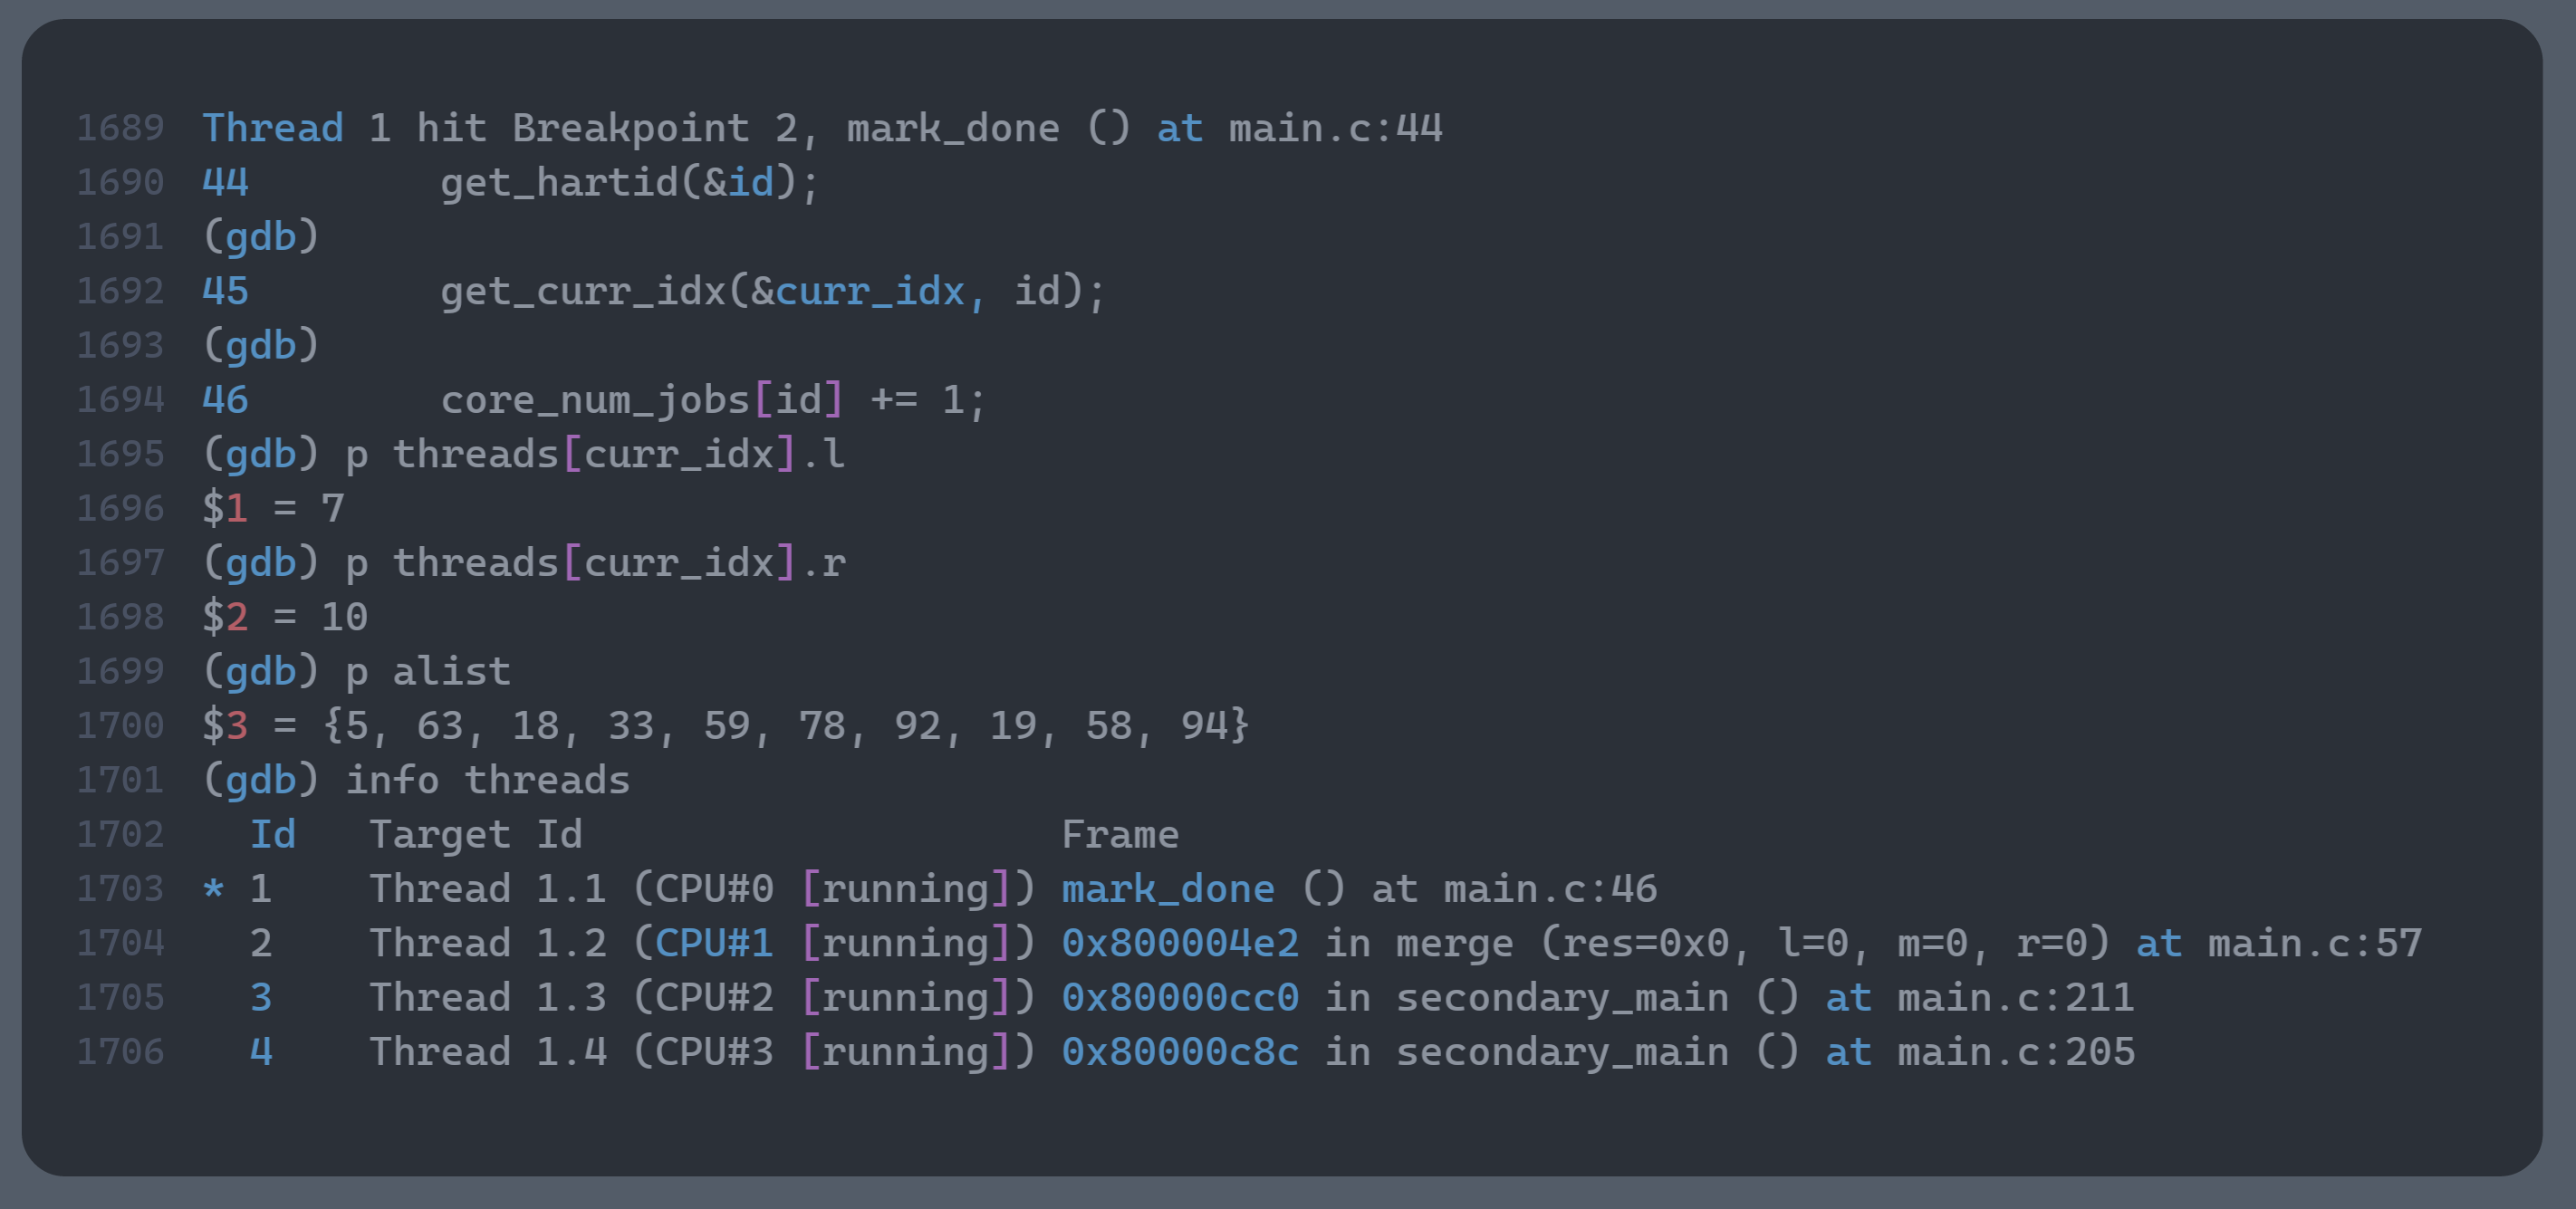
\includegraphics[width=\textwidth]{./figures/debug2.png}
    \caption{Hit breakpoint, where alist is sorted by core 1 from
    index 7 to 10 (10 exclusive).}
  \end{subfigure}
  \caption{Debugging the QEMU virtual machine with 4 cores.}\label{fig:debug}
\end{figure}

To access and debug the multicore system, QEMU provides a way for a remote
gdb-server to connect at the start of execution\cite{QEMU}. In a system where
each core is equivalent, gdb will automatically detect the cores, but will
display them as threads. This allows one to debug the QEMU virtual machine with
the same methodology used when debugging multithreaded execution. The workflow
shown in Figure~\ref{fig:debug} is as follows:
\begin{itemize}
\item Change directory to src/bare\_metal.
\item Initialize the alist.c file with an array and a given size.
\item "make clean" to remove any previous build.
\item Run "make debug" to initialize the QEMU virtual machine.
\item In a separate terminal instance run "riscv32-unknown-elf-gdb". This will
  automatically run the commands in the ".gdbinit" file and connect to the QEMU
  virtual machine.
\item Break at mark\_done. This function is run whenever a given thread job is
  finished.
\item Run "info threads" to get an overview of all threads.
\end{itemize}
As an example, Figure~\ref{fig:debug} shows a list of size 10, where core 1 has
sorted the subsection of the list from index 7 to 10. This section corresponds
to one fourth of the list, as the number of cores available is 4.

\subsection{Validation}\label{sec:validate}
\begin{table}
  \caption{Table of tests run}\label{tab:tests}
  \begin{center}
    \begin{tabular}[c]{l|l|l|l|l|l|l}
      & \multicolumn{6}{c}{NUM\_CORES}\\
      \cline{2-7}
      Lower:Upper:Number & 2 & 4 & 8 & 16 & 32 & 64\\
      \hline
      -100:0:100 & pass & pass & pass & pass & pass & pass \\
      \hline
      0:100:100 & pass & pass & pass & pass & pass & pass\\
      \hline
      -50:50:100 & pass & pass & pass & pass & pass & pass \\
      \hline
      -50:50:10 & pass & pass & pass & fail & fail & fail \\
      \hline
      -1000:1000:1000 & pass* & pass* & pass* & pass* & pass* & pass* \\
      \hline
      -1000:1000:20000 & pass* & pass* & pass* & pass* & pass* & pass* \\
      \hline
      -1000:1000:100000 & pass* & pass* & pass* & pass* & pass* & pass* \\
    \end{tabular} \\
    \vspace{1em}
    \raggedright{\footnotesize *This run initially failed due to stack overflow.
    After increasing the different stack sizes following Appendix~\ref{ap:stack}
  it passed.} \\
  \end{center}
\end{table}

When running a test, the .elf file first prints the unsorted array, and then
once sorting is done, prints it again. When executing "make test", the QEMU
virtual machine outputs the stdout to a file called test.txt. Subsequently,
invoking "python3 validate.py" reads this file to ascertain if sorting was
performed correctly. In Table 6, an overview of some tests I conducted can be
seen. On the left, the formatting is specified as the lower bound of randomly
selected numbers, the upper bound, and the number of random elements in the
list. A value of 'pass' signifies that the validate.py file executed without
throwing an assertion error. A value of 'fail' signifies that validate.py threw
an error when running. The tests were initially performed with a global stack of
0x800,\footnote{defined in ram.ld. Equates to 2048 bytes.} a STACK\_SIZE of 2048
bytes and a THREAD\_STACK\_SIZE of 1024 bytes. If a failure occurred,
modifications were made to these three values in an attempt to pass the test.

In Table~\ref{tab:tests} one can see that when the number of cores is greater than
the number of elements in the list it fails executing the sorting algorithm.
Generally it would not seem relevant to ever run a merge sort algorithm with
more cores than there are elements in the list due to the tree structure created
with merge sort. The error is caused by the merge function being told to merge a
single element, which is undefined behaviour in the current implementation. I
have decided not to leave a check for this, and instead assume that the number
of cores is never larger than the length of the input list.

\subsection{Future work}
The implementation proposed in this thesis is more a proof of concept, and as
such comes with a few shortcomings. Firstly, with the current implementation
there is a heavy reliance on the GLOBAL\_STACK\_SIZE. The array to be sorted is
hard-coded and stored on the global stack, which can occupy substantial space
when dealing with large arrays. Furthermore, the array of thread jobs is also
saved on the global stack. With the current implementation each thread type has
a size of 848 bytes. Thus, a solution that reduces overall usage of the global
stack, or a better method of detecting the size of the global stack would allow
for a more reliable solution.

Whenever a merge sort splits the array into two halves, there is created a new
thread with an allocated stack size of THREAD\_STACK\_SIZE. The top-level thread
job, which has to sort the entire array, must first create a copy of the array
before it can sort in place. The same goes for all other thread jobs, but the
amount of the array they need to copy is halved for each level moved down in the
merge sort tree shown in Figure~\ref{fig:mergesort}. In theory, this allows for
halving the size of the allocated thread stack for each level change. This does
not take into account the constant space needed for the declared variables, so
the thread stack size might instead be represented by:
\begin{align}
  \text{THREAD\_STACK\_SIZE} = \text{INITIAL\_STACK\_SIZE} / 2^i + C
\end{align}
Where i is the depth level, and C is some constant used to store the variables
needed during computation, this constant C would then be different depending on
whether the given thread has to perform merge sort or just merge over the array.
Experiments determining the size of C could be carried out to optimize
memory better.

Furthermore, with the current implementation core 0 is the only thread writing
to the global threads array. This core is tasked with initializing all the
threads jobs, which means that all other cores must wait until this single
thread has finished its initialization. As the number of cores grows, so does
the time it takes to initialize the threads. This is inherently inefficient. As
such future work could propose a solution where the work of initializing the
threads array could be spread among multiple cores instead.

As the implementation is carried out using QEMU, it is not possible to do
performance testing. Firstly, the implementation is implemented on bare-metal,
and would need some sort of custom timing implemented to get the time at the
start and then at the end. Secondly, as QEMU is a virtual machine, it mimics
multiple cores by creating threads on the host pc. These threads provide an
illusion of multicore, but the host operating system is still in charge of
scheduling, which performance vice removes any theoretical performance by
creating the bare-metal design in the first part. For performance testing the
implementation must be carried out on actual hardware, such that it is not just
a virtualisation of the bare-metal platform.

The implementation also requires that the number of cores is a power of 2. This
is due to how the initialization builds the threads up. This issue has a few
ways it can be fixed. Firstly, instead of stopping at the same level for all the
merge sorts, it could theoretically split only a few of the sublists given,
such that instead of having to be a power of 2, it would instead only require
that it is a multiple of 2. This would still allow for all cores to work on a
sublist at the same time. Another approach would be to allow a subset of the
number of cores to busy loop until the two child threads finish as described in
Section~\ref{sec:init_threads}. The former approach seems more promising, but is
left as something which can later be addressed.

As it stands, the only method of loading an array onto the processor is by hard
coding the list into the .elf file. Although this works to show the entire
sorting algorithm, it would not be useful in an actual data center unless some
sort of communication protocol is established between the host CPU and the
computational storage device. I have left this communication up for future work.

